\chapter{Adquisición de datos}

Esta clase tiene como objetivo comprender los pasos básicos para adquirir imágenes satelitales. Se utilizará el catálogo \emph{United Stated Geological Service (USGS)}.

\section{Descarga de imágenes}

Para iniciar la adquisición de imagenes deberá registrarse el sitio web del \href{https://earthexplorer.usgs.gov/}{USGS}\footnote{\href{https://earthexplorer.usgs.gov/}{https://earthexplorer.usgs.gov/}}.

Una vez que ingresa con su usuario y contraseña, en el margen superior izquierdo encontrará los componentes de búsqueda, dividido en cuatro solapas. En \texttt{Seach Criteria} seleccione \texttt{Address/Place}, escriba \texttt{Iguazú} y presione \menu{Show} (Figura \ref{fig:busqueda}).

\begin{figure}[h!]
    \centering
    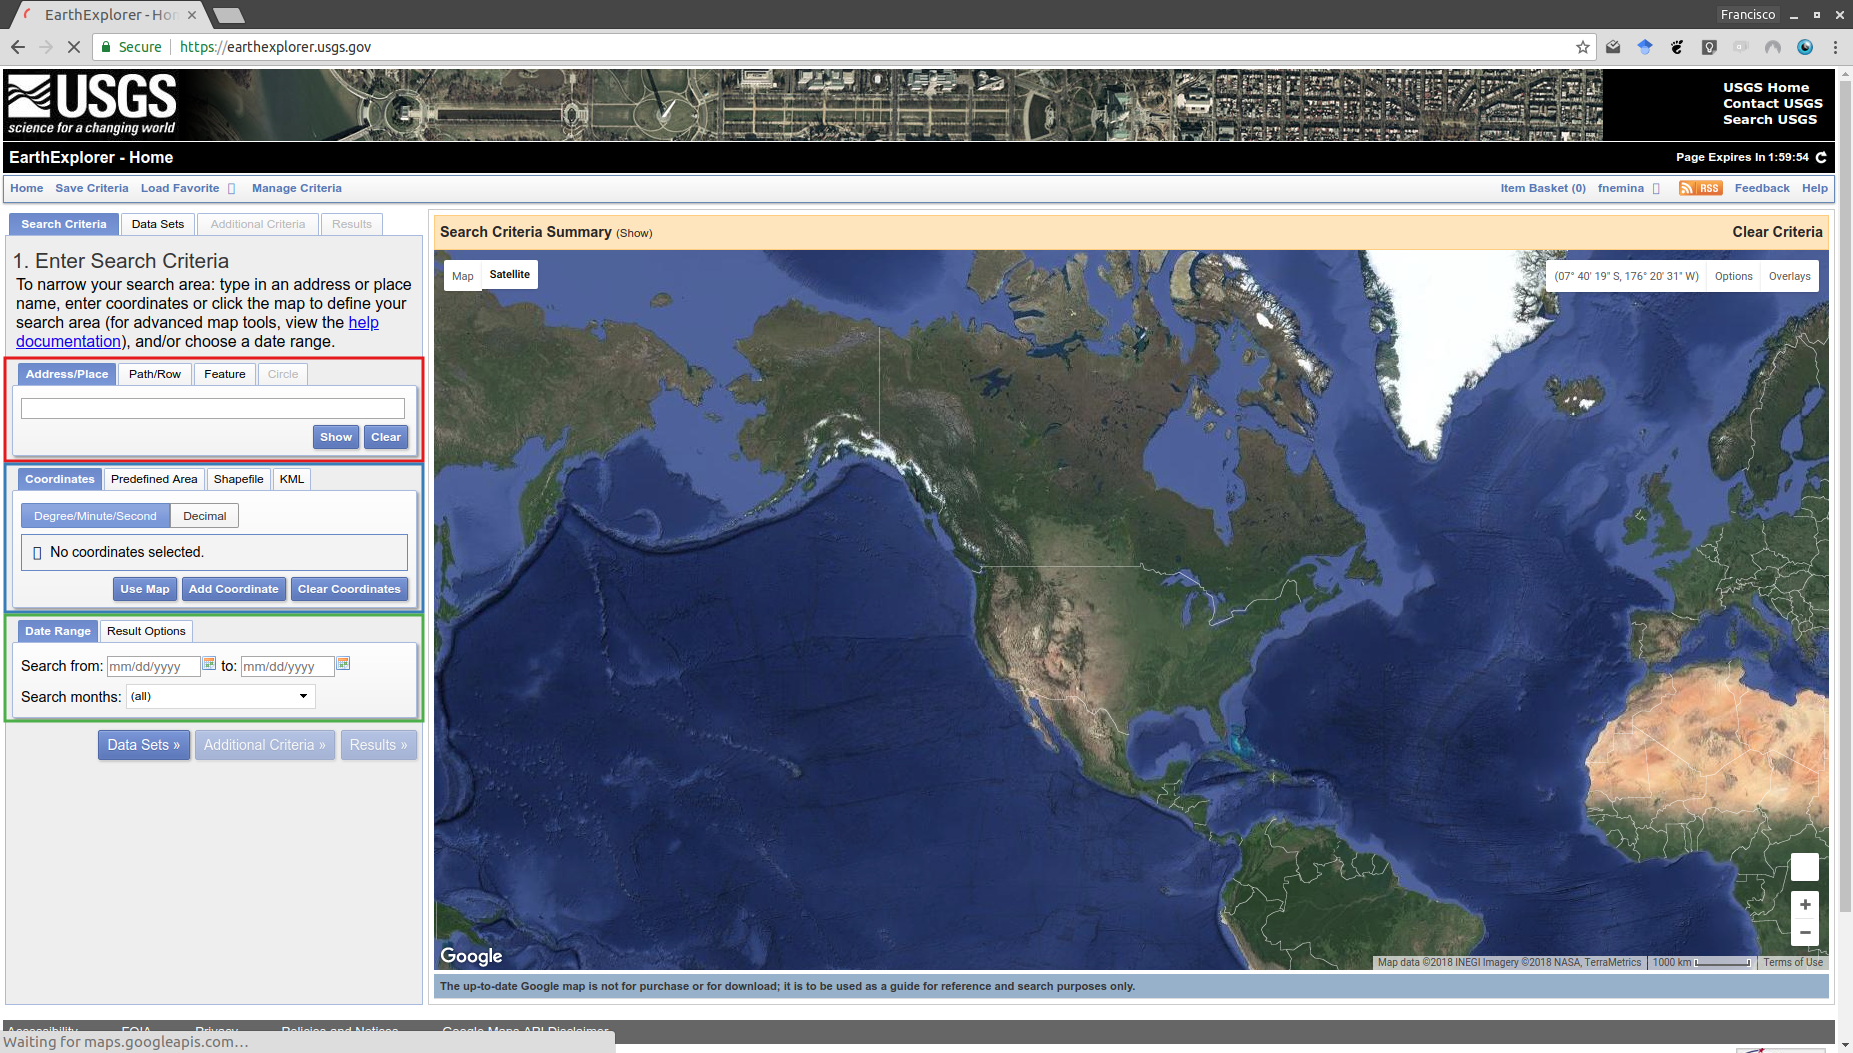
\includegraphics[width=0.6\textwidth]{fig:busqueda.png}
    \caption{Busqueda en el catálogo del \emph{USGS}. Puede observarse el sector de busqueda en rojo, el sector de área en azul y el sector de selección temporal en verde.}
    \label{fig:busqueda}
\end{figure}

Haga click sobre el nombre \texttt{Misiones Province, Argentina} y se mostrará la zona en el mapa. 

La opción \menu{Data Range} permite definir un rango de tiempo dentro de la búsqueda. Indique la fecha desde el 1 de julio de 2017 hasta el 31 de julio de 2017, deplegando el calendario y haciendo click sobre el número correspondiente.

En la solapa \menu{Data Sets} encontrará la lista de satélites disponibles. En el recuadro \texttt{Data Set Search:} escriba \texttt{Landsat 8} y seleccione del menú la opción \texttt{Landsat 8 OLI/TIRS C1 Level-2} (Figura \ref{fig:dataset}). Para finalizar presione \menu{Results}.

\begin{figure}[h!]
    \centering
    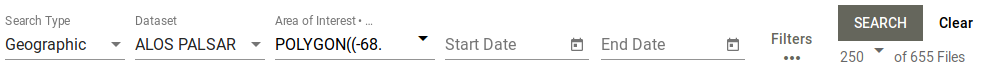
\includegraphics[width=0.6\textwidth]{fig:dataset.png}
    \caption{Selección de un set de datos en el catálogo del \emph{USGS}. Puede observarse el área de busqueda en rojo y el satelite selecccionado en el recuadro verde.}
    \label{fig:dataset}
\end{figure}

A la izquierda de la pantalla aparecerá una lista de productos. Busque el correspondiente al 13 de julio del 2017, del path 224 y row 78. Haga click sobre \menu{Order scene} (Figura \ref{fig:descarga}-b).

\begin{figure}[H]
    \centering
    \subfloat[]{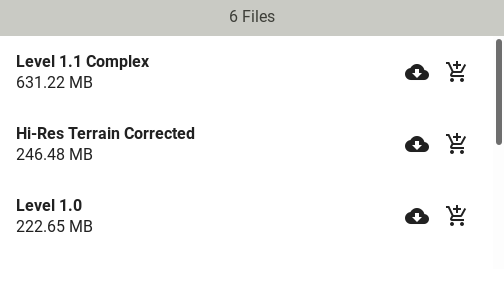
\includegraphics[width=0.6\textwidth]{fig:descarga.png}}
    \\
    \subfloat[]{
\includegraphics[scale=0.5]{fig:operaciones.png}}
    \caption{a) Productos disponibles para la descarga en el catálogo del \emph{USGS}. En rojo se destaca el botón para ver el pedido. b)Herramientas del catálogo. De izquierda a derecha: Footprint, Show Browse Overlay, Compare Browse, Show Metadata and Brose, Order Scene y Exlude escene from Results.}
    \label{fig:descarga}
\end{figure}

Para corroborar el pedido haga click en \menu{View Item Basket} y luego en \menu{Proceed to Checkout}. Finalice presionando \menu{Submit Order}.

La imagen solicitada pertenece a una serie de productos a demanda.  Cuando  esté disponible su descarga, le enviarán un correo electrónico notificándolo \footnote{Recibirá 3 correos electrónicos en total: dos confirmando el pedido y uno cuando la descarga esté disponible}. El asunto será

\begin{center}
\texttt{USGS ESPA product request order number [] available for download}
\end{center}

entre \texttt{[]} estará el número de pedido. Ingrese al link que figura en el correo recibido y, en la nueva página, seleccione su pedido en la columna \texttt{Order ID}. Descargue la imagen presionando \texttt{Download}.

\begin{figure}[h!]
    \centering
    \subfloat[]{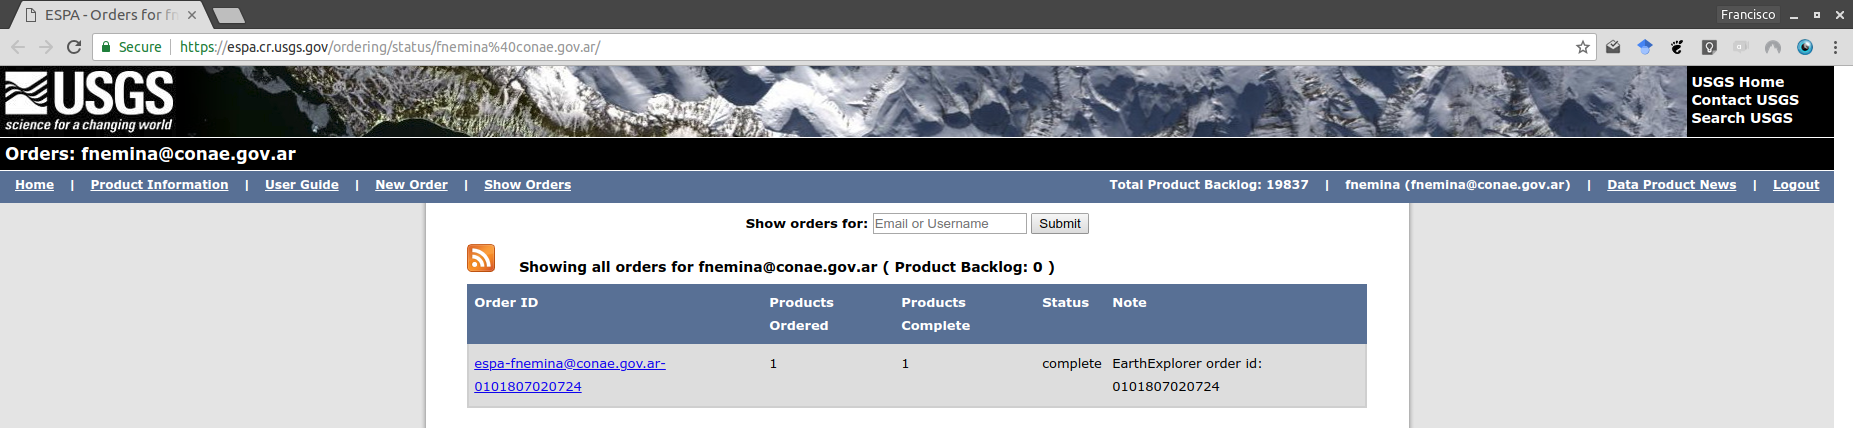
\includegraphics[width=0.6\textwidth]{fig:descarga2.png}}
    \\
    \subfloat[]{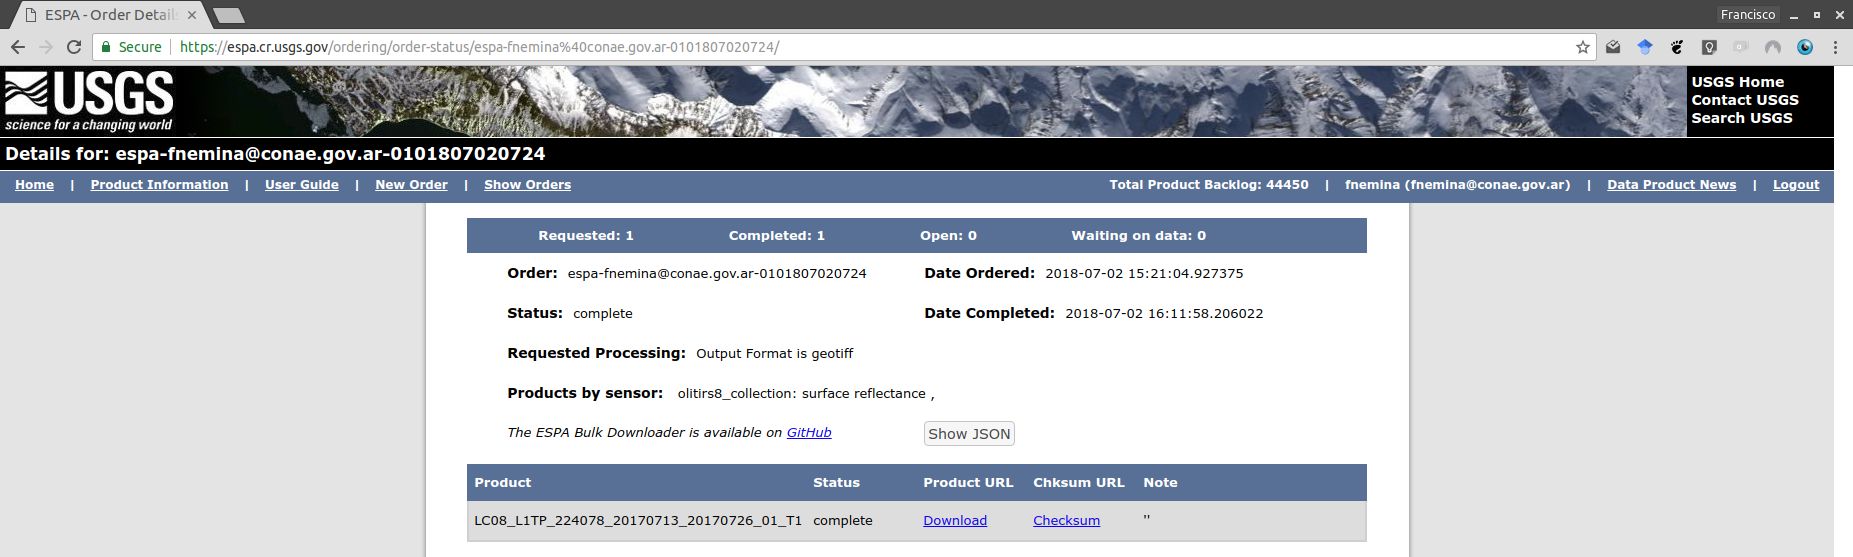
\includegraphics[width=0.6\textwidth]{fig:descarga3.png}}
    \caption{Descarga de productos.}
    \label{fig:descarga2}
\end{figure}

\textbf{Observación:} El producto puede demorar hasta 48 horas para estar disponible.

Una vez finalizada la descarga descomprima el archivo. Necesitará un descompresor como winrar, 7zip o similar.

\section{Apilado de bandas}
Dentro de la carpeta descomprimida, las bandas de la imagen se encuentran en archivos separados

\begin{center} \directory{LC08\_L1TP\_224078\_20170713\_20170726\_01\_T1\_sr\_band1},
\end{center}
\begin{center} \directory{LC08\_L1TP\_224078\_20170713\_20170726\_01\_T1\_sr\_band2},
\end{center}
\begin{center} \directory{LC08\_L1TP\_224078\_20170713\_20170726\_01\_T1\_sr\_band3},
\end{center}
\begin{center} \directory{LC08\_L1TP\_224078\_20170713\_20170726\_01\_T1\_sr\_band4},
\end{center}
\begin{center} \directory{LC08\_L1TP\_224078\_20170713\_20170726\_01\_T1\_sr\_band5},
\end{center}
\begin{center} \directory{LC08\_L1TP\_224078\_20170713\_20170726\_01\_T1\_sr\_band6}
\end{center}
\begin{center} y \directory{LC08\_L1TP\_224078\_20170713\_20170726\_01\_T1\_sr\_band7}.
\end{center}

Abra todos los archivos en SNAP y podra visualizar cada banda por separado

Vaya a \menu{Radar > Coregistration > Stack tools > Create Stack} y en la pestañá \menu{1-ProductSet-Reader} haga click en \menu{Add oppened}. Ordene las bandas según su número. Seleccione una banda y con los botones \menu{Move up} y \menu{Move down} cambie su posición (Figura \ref{fig:stack1}).

En la pestaña \menu{2-CreateStack} seleccione la opción \emph{Product Geolocation} para el parámetro \menu{Initial Offset method} (Figura \ref{fig:stack2}).

Finalmente en la pestaña \menu{3-Write} escriba el nombre del archivo de salida y la carpeta donde se guardarán los datos. Haga click en \menu{Run} y se creara un archivo .dim y el resultado se agregará al \emph{Product explorer}(Figura \ref{fig:stack3}).

\begin{figure}[h!]
    \centering
    \subfloat[1-ProductSet-Reader]{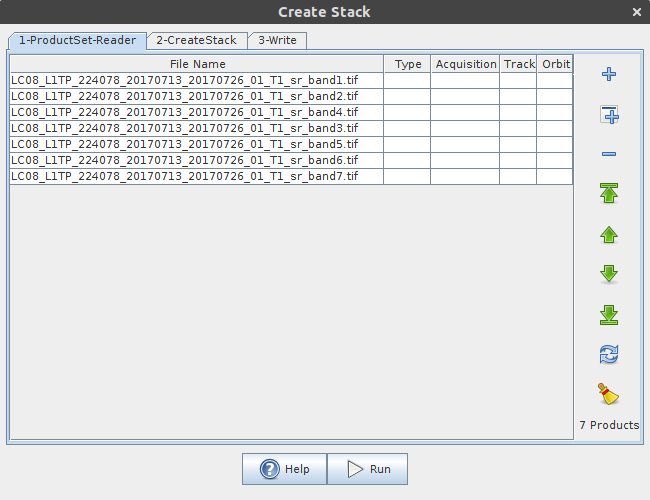
\includegraphics[width=0.4\textwidth]{fig:stack1.png}\label{fig:stack1}}
    \hspace{1cm}
    \subfloat[2-CreateStack]{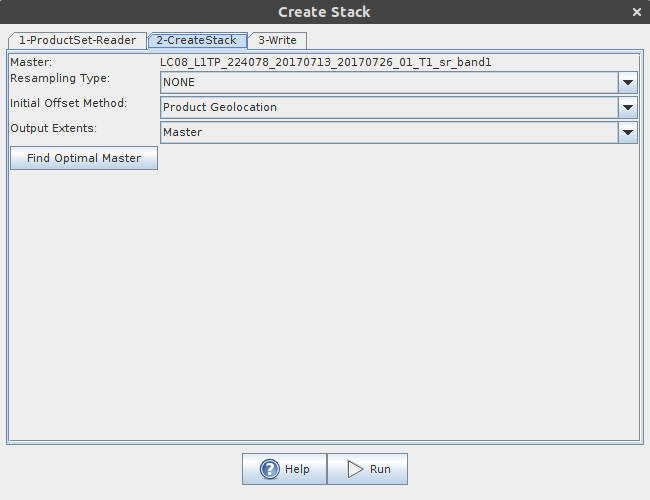
\includegraphics[width=0.4\textwidth]{fig:stack2.png}\label{fig:stack2}}\\
    \subfloat[3-Write]{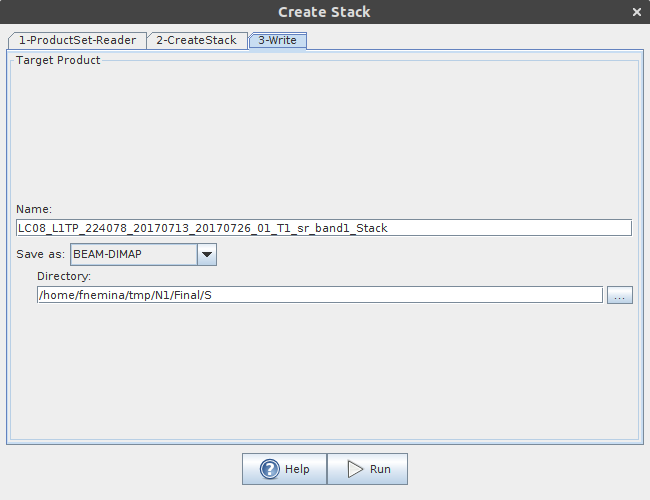
\includegraphics[width=0.4\textwidth]{fig:stack3.png}\label{fig:stack3}}
    \caption{Apilado de productos en el SNAP usando la herramienta \menu{Create Stack}.}

\end{figure}

\section{Propiedades de la imagen}
Es de utilidad editar las propiedades de la imagen para agregar los nombres de las bandas, su longitud de onda central y tipo de dato.

Haga doble click en el nombre de la imagen y despliegue la carpeta de bandas. Luego, con click derecho sobre
\begin{center}
\texttt{band\_1\_mst\_01Jan2000}
\end{center}
seleccione \menu{Properties} de la lista. En al ventana que se despliega es posible cambiar el nombre de la banda, la unidad de medida, el valor digital no válido, la longitud de onda central y el ancho de la banda (Figura \ref{fig:prop}).

\begin{figure}[h!]
    \centering
    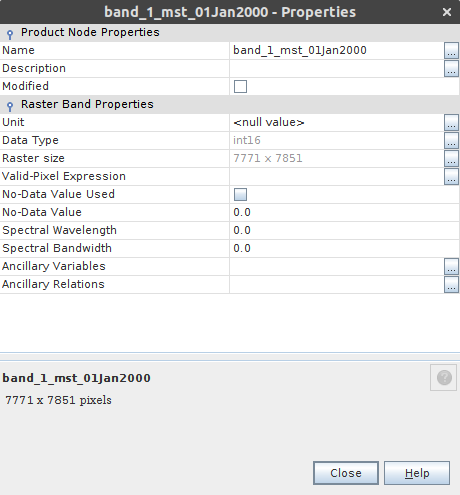
\includegraphics[width=0.35\textwidth]{fig:prop.png}
    \caption{Propiedades de una banda de la imagen.}
    \label{fig:prop}
\end{figure}

Edite el campo \emph{Name} con el texto \texttt{ca} y el campo \emph{Spectral Wavelength} con el valor \texttt{442}. Repita el mismo procedimiento para el resto de las bandas utilizando los datos que figuran en la Tabla \ref{tab:landsat8}.

\begin{table}[h!]
  \centering
  \begin{tabular}{@{}lclc@{}}
  \toprule
  Bands designation          & Número & Name  & Wavelength {[}nm{]} \\ \midrule
  Aerosoles costeros         & 1      & ca    & 442                 \\
  Azul                       & 2      & blue  & 482                 \\
  Verde                      & 3      & green & 561                 \\
  Rojo                       & 4      & red   & 655                 \\
  Infrarrojo cercano         & 5      & nir   & 865                 \\
  Infrarrojo de onda corta 1 & 6      & swir1 & 1610                \\
  Infrarrojo de onda corta 2 & 7      & swir2 & 2200                \\ \bottomrule
  \end{tabular}
\caption{Nombre y longitud de onda de cada banda para el producto Landsat 8 - level 2 collection.}
\label{tab:landsat8}
\end{table}

Guarde los cambios realizados. Haga click derecho sobre el nombre de la imagen y seleccione \menu{Save product}.

\section{Subset espacial y espectral}
Para reducir el tamaño de la imagen y los tiempos de procesamiento, es posible hacer un recorte o subset espacial y espectral de la zona de interes.

Seleccione la imagen apilada y diríjase a \menu{Raster > Subset}, allí se abrirá una nueva ventana. En la pestaña \menu{Spatial subset} elija \menu{Geo Coordinates} (Figura \ref{fig:subset}).

\begin{figure}[h!]
    \centering
    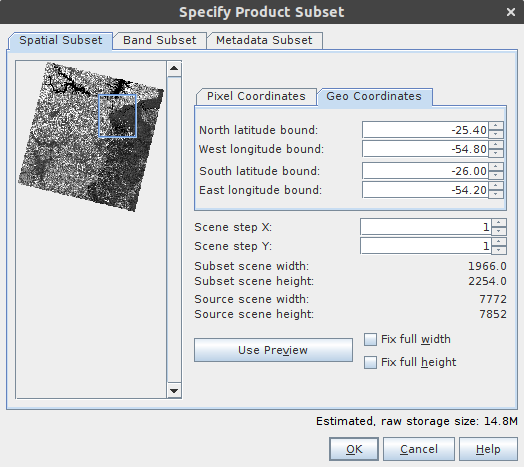
\includegraphics[width=0.45\textwidth]{fig:subset.png}
    \caption{Subset espacial de una imagen Landsat 8 utilizando coordenadas geográficas.}
    \label{fig:subset}
\end{figure}

Recorte la imagen ingresando las coordenadas geográficas:

\begin{itemize}
    \item North latitude bound: -25.4
    \item West longitude bound: -54.8
    \item South latitude bound: -26.0
    \item East longitude bound: -54.2
\end{itemize}

Finalice presionando \menu{Ok}. Haga click derecho sobre el nombre y seleccione  \menu{Save Product}, para guardar el recorte.



\section{Reproyección}
En algunas aplicaciones, la proyección por defecto que contiene la imagen, podría no ser la adecuada. Cambie la proyección desde: \menu{Raster > Geometric operations > Reprojection} (Figura \ref{fig:repro}). 

\begin{figure}[h!]
    \centering
    \subfloat[I/O Parameters]{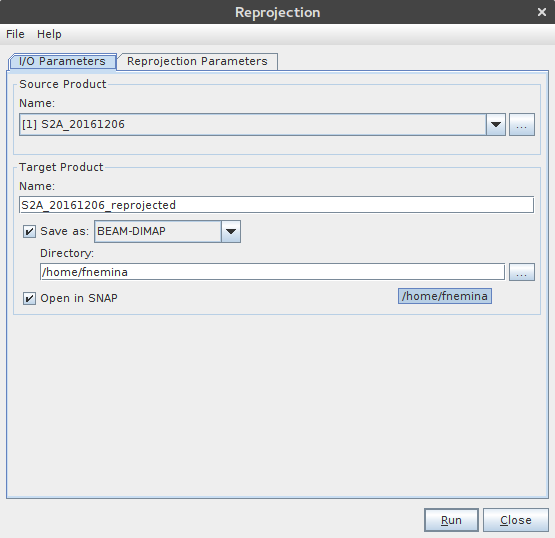
\includegraphics[width=0.4\textwidth]{fig:reproj1.png}}
    \hspace{1cm}
    \subfloat[Processing parameters]{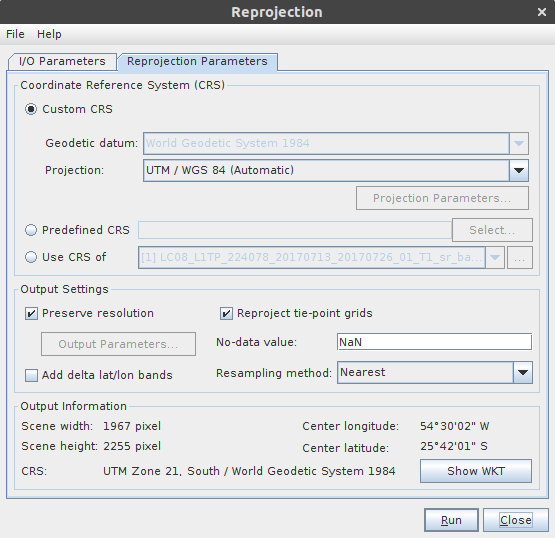
\includegraphics[width=0.4\textwidth]{fig:reproj2.png}}
    \caption{Herramienta de reproyección. La imagen se proyecta en coordenadas geográficas.}
    \label{fig:repro}
\end{figure}

En \menu{I/O parameters}, utilice la imagen recortada como entrada en \menu{Sourse product}. Luego, escriba el nombre del archivo de salida e indique la carpeta de guardado. Llame a la nueva imagen:

\begin{center}
  \directory{LC08\_224-078\_2017-07-13.dim}
\end{center}

En la pestaña \menu{Reprojection parameters} elija la opción \emph{Custom CRS} y en el menú desplegable de Projection busque\emph{UTM / WGS 84 (automatic)}. De esta forma la imagen será reproyectada a la faja correspondiente del sistema de coordenadas \emph{UTM/WGS84}. Haga click en \menu{Run} para finalizar.

\section{Actividad práctica}

\begin{enumerate}
  \item Identifique en la imagen descargada:
  \begin{enumerate}
    \item El río Iguazú.
    \item El río Paraná.
    \item La ciudad de Puerto Iguazú.
    \item La zonas cultivadas al norte del río Iguazú.
    \item Las zonas cultivadas al oeste del río Paraná.
    \item La selva Paranaense.
    \item El embalse Urugua-í al sur de la imagen.
    \item La zona de forestaciones.
    \item El Aeropuerto Cataratas del Iguazú.
  \end{enumerate}
  ¿Qué combinación de bandas conviene utilizar para obtener mejores resultados?

  \item Obtenga una firma espectral de:
  \begin{enumerate}
    \item El río Iguazú.
    \item El río Paraná.
    \item El embalse Urugua-í.
    \item La selva paranaense.
    \item Una forestación.
    \item Suelo con cultivo.
    \item Suelo en descanso.
  \end{enumerate}

  \item Compare visualmente la imagen Landsat 8 del 5 de enero de 2018 y del 13 de julio de 2017. Elija la combinación de bandas que considere adecuada. 
  \begin{enumerate}
    \item ¿Qué observa sobre el río Paraná e Iguazú?.
    \item ¿Qué observa sobre la selva paranaense?.
    \item ¿Qué  observa en la zona de forestaciones?.
    \item ¿Qué  observa en la zona de cultivos?.
  \end{enumerate}
  ¿En qué se parecen? ¿Qué coberturas cambian de color para las dos imágenes?

  \item Compare las firmas espectrales obtenidas de la imagen Landsat 8 del 5 de enero de 2018 y del 13 de julio de 2017.
  \begin{enumerate}
    \item Sobre el río Paraná.
    \item Sobre el río Iguazú.
    \item Sobre la selva Paranaense.
    \item Sobre las forestaciones.
    \item Sobre un mismo parche de cultivo.
  \end{enumerate}
  ¿Qué observa en el comporamiento de las firmas espectrales? ¿A qué cree que se debe? ¿Cómo lo explicaría en funsión de las propiedades biofísicas de cada cobertura?
\end{enumerate}

Estas preguntas y actividades no serán evaluadas. Su objetivo es discutirlas en el foro de consultas e intercambio de la clase.
